\cleardoublepage % memastikan bab baru dimulai di halaman ganjil (kanan)
\chapter{STUDI LITERATUR}
\label{chap:studi-literatur}
\section{Tumor Otak}
Berdasarkan \textcite{mayo2023brain}, tumor otak didefinisikan sebagai pertumbuhan abnormal sel yang terjadi di dalam atau di dekat otak. Lokasi tumor dapat bervariasi, mencakup jaringan otak, saraf, kelenjar pituitari, kelenjar pineal, serta membran yang menutupi permukaan otak. Tumor yang bermula di otak disebut tumor otak primer, sedangkan tumor yang menyebar ke otak dari bagian tubuh lain disebut tumor otak sekunder atau metastatik.

\subsection{Teknologi Pencitraan Medis Tumor Otak}

Langkah awal untuk mendiagnosis tumor otak adalah pemeriksaan fisik, tes penglihatan, riwayat medis, dan tes neurologis untuk mengevaluasi fungsi otak serta saraf. Jika tes awal menunjukkan kemungkinan adanya tumor otak, pencitraan diagnostik akan dilakukan dan dianalisis oleh ahli neuroradiologi \autocite{farber2025how}. Dalam pencitraan tumor otak, terdapat tiga bidang utama yang bisa dilakukan oleh alat pencitraan seperti pada Gambar \ref{gambar:gambartumor} \autocite{hartung2023abdominal}.

\begin{figure}[h]
	\centering
	\captionsetup{justification=centering}
	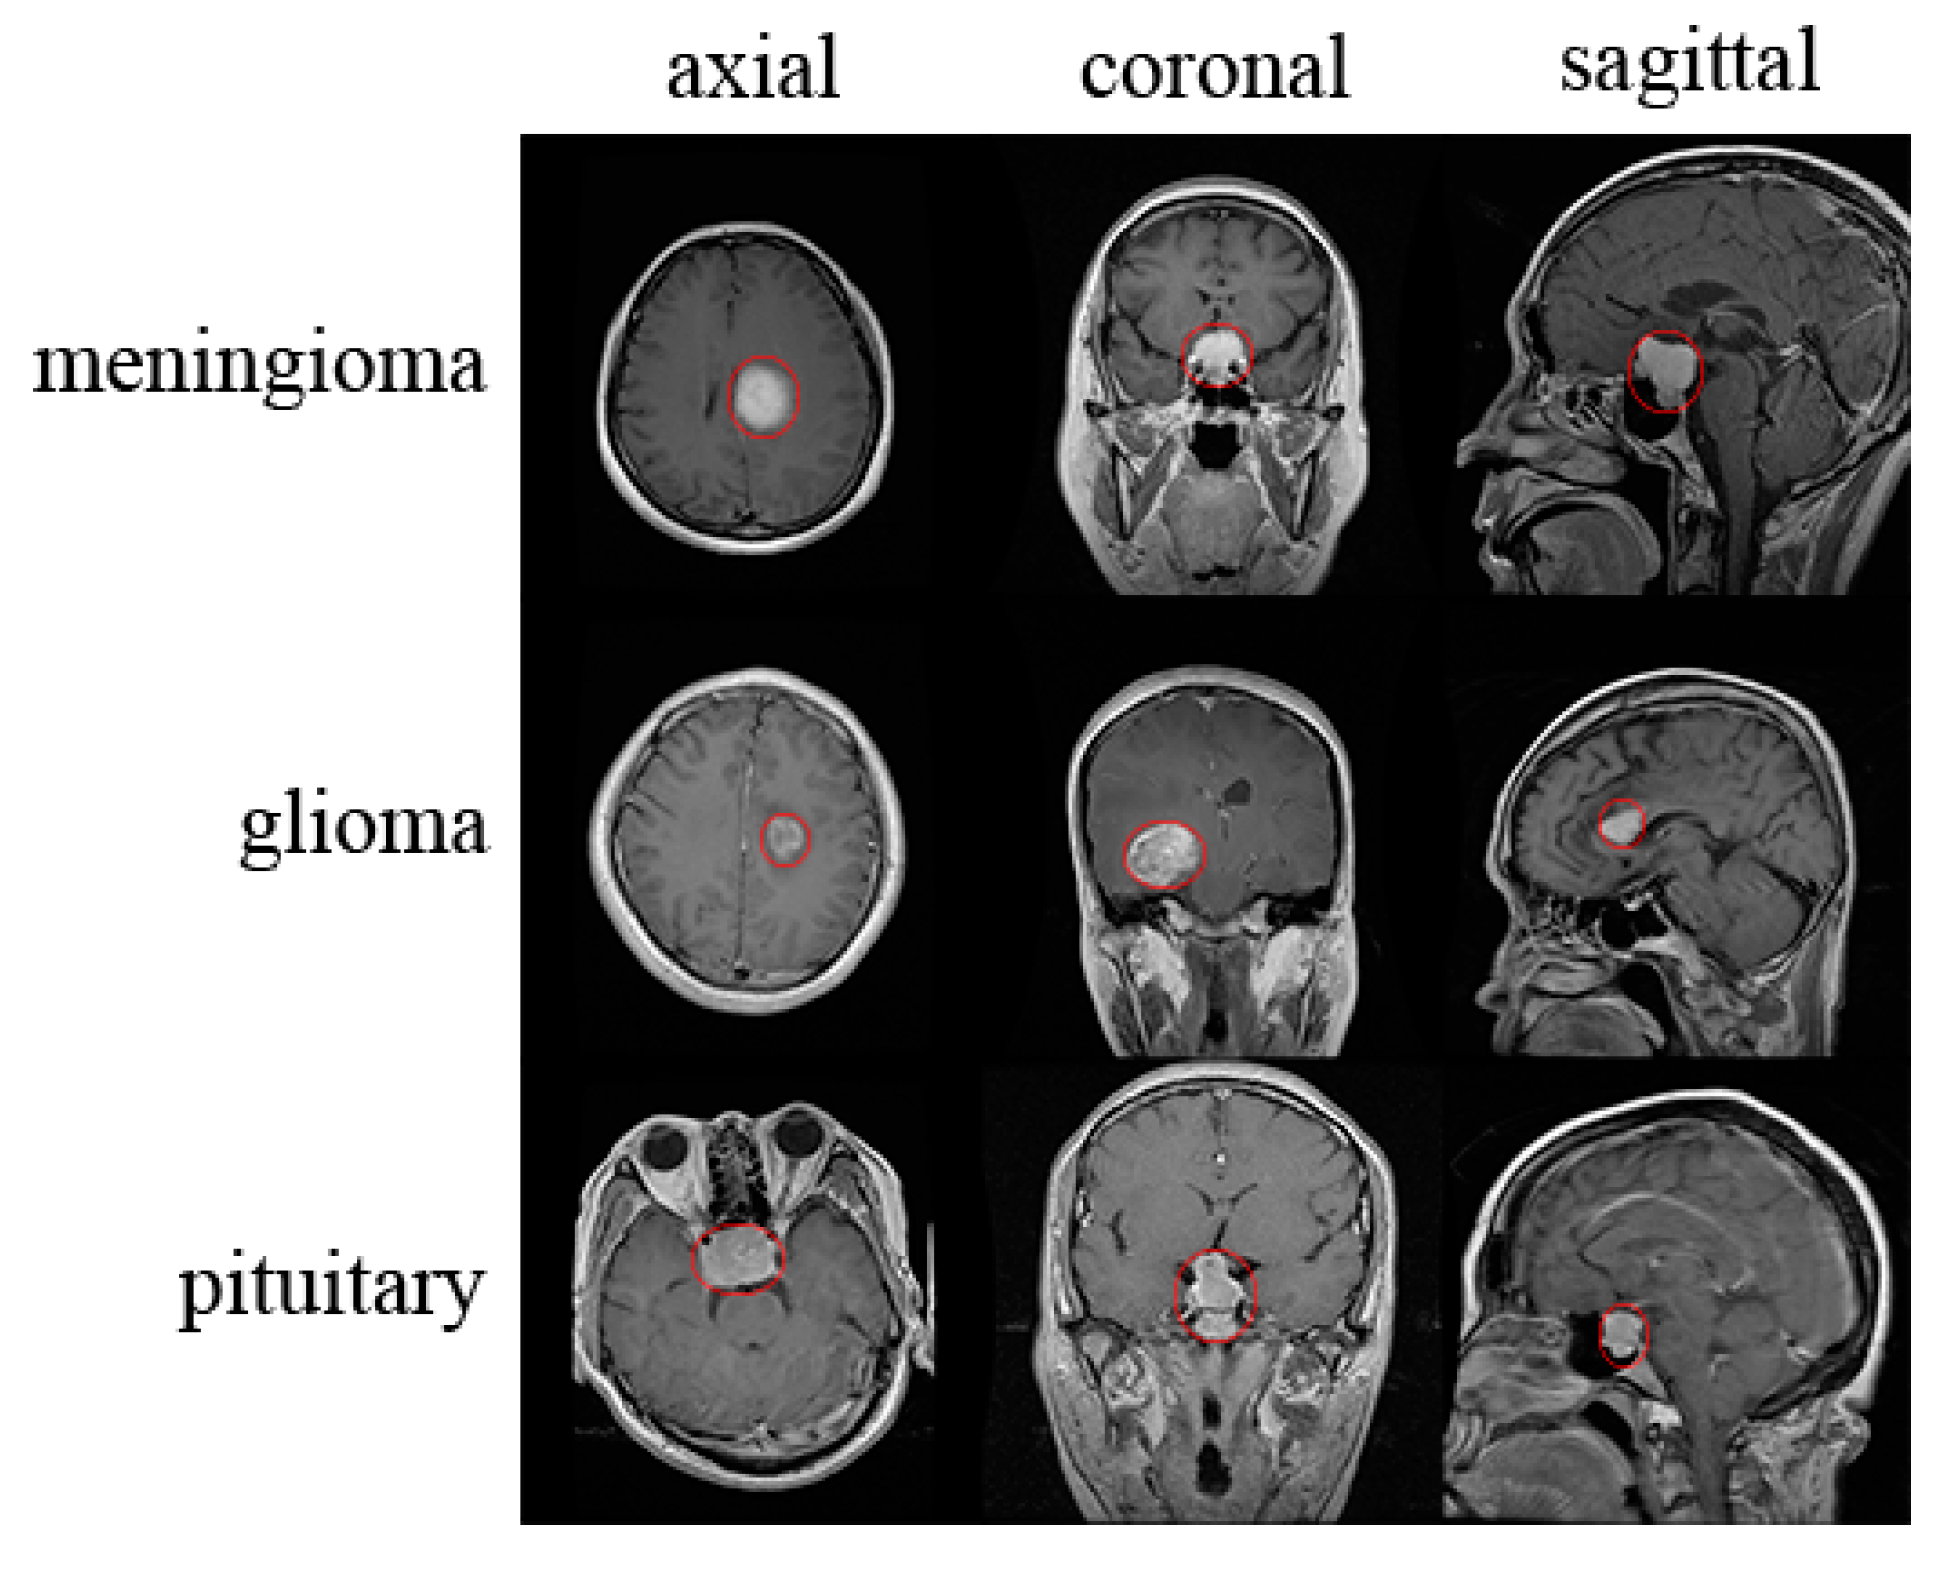
\includegraphics[width=0.7\textwidth]{images/gambartumor.png}
	\caption{\textit{CT Scan} Otak 
		\autocite{kamesh2024brain}}
	\label{gambar:gambartumor}
\end{figure}

Berdasarkan \textcite{radiologykey2015brain}, terdapat tiga bidang dalam pencitraan medis.
\begin{enumerate}
	\item Bidang Aksial\\
	Bidang aksial yang juga sering disebut sebagai bidang \textit{transverse} merupakan bidang horizontal yang memotong tubuh secara melintang sehingga membaginya menjadi bagian atas dan bagian bawah. Bidang ini dinamakan aksial karena orientasi bidang ini posisinya tegak lurus terhadap sumbu panjang atau poros utama tubuh manusia. Dalam konteks medis seperti \textit{CT Scan}, bidang ini memungkinkan dokter melihat irisan tubuh seolah-olah dilihat dari arah kaki ke arah kepala atau sebaliknya.
	\item Bidang Koronal \\
	Bidang koronal atau dikenal juga sebagai bidang frontal adalah bidang vertikal yang membelah tubuh menjadi dua bagian, yaitu bagian depan dan bagian belakang. Bidang ini dinamakan koronal karena bidang ini berjalan sejajar dengan \textit{coronal suture} pada tengkorak manusia. Sutura ini adalah garis pertemuan tulang tengkorak yang posisinya menyerupai letak mahkota di atas kepala, atau seperti bando yang melintang dari telinga kiri ke telinga kanan.
	\item Bidang Sagital \\
	Bidang sagital merupakan bidang vertikal yang memisahkan tubuh menjadi sisi kanan dan sisi kiri. Bidang ini dinamakan sagital karena posisinya sejajar atau melewati sutura tersebut, yang secara visual menyerupai bentuk atau arah anak panah yang melesat lurus jika dilihat dari arah depan wajah.
\end{enumerate}

\subsubsection{MRI}
\textit{Magnetic Resonance Imaging} (MRI) merupakan teknologi pencitraan 3D noninvasif beresolusi tinggi yang memanfaatkan interaksi medan magnet kuat dan gelombang radio terhadap proton dalam molekul air pada jaringan tubuh. Berdasarkan perbedaan waktu relaksasi energi proton tersebut, MRI sangat unggul untuk memvisualisasikan detail anatomi jaringan lunak—seperti struktur otak, saraf, dan otot—serta efektif dalam mendiagnosis tumor tanpa paparan radiasi. Meskipun aman dari radiasi, penggunaannya dikontraindikasikan bagi pasien dengan implan logam (misalnya alat pacu jantung) dan memiliki risiko penyerta seperti kebisingan, stimulasi saraf, hingga potensi toksisitas agen kontras gadolinium pada penderita gangguan ginjal \autocite{nibib2025mri}.

\subsubsection{CT Scan}
\textit{Computed Tomography} (CT) adalah prosedur pencitraan diagnostik yang menggunakan teknologi sinar-X. Prosedur ini bekerja dengan mengarahkan berkas sinar-X yang sempit dan berputar cepat mengelilingi tubuh pasien. Sinyal yang dihasilkan kemudian diproses oleh komputer untuk membuat serangkaian gambar irisan tomografi secara detail, yang dapat direkonstruksi menjadi gambar tiga dimensi (3D).

CT Scan memiliki peran penting sebagai instrumen peringatan dini dalam mendiagnosis tumor otak. Berdasarkan penelitian oleh \textcite{budiman2024effectiveness}, penggunaan CT Scan terbukti sangat efektif dan memberikan dampak positif bagi deteksi dini tumor otak pada manusia. Tingkat efektivitas ini dibuktikan secara kuantitatif melalui perolehan nilai rata-rata effect size sebesar 1.17 yang masuk dalam kategori tinggi. Selain itu, hasil pengujian N-Gain juga menunjukkan skor 0.58 dengan kategori efektivitas tinggi.

Meskipun MRI sering dianggap sebagai metode pencitraan yang lebih sensitif dalam mendeteksi keberadaan tumor yang berukuran kecil, CT Scan tetap menawarkan keunggulan lain, seperti tingkat ketersediaan alat yang lebih merata di berbagai fasilitas kesehatan serta waktu pemeriksaan yang jauh lebih singkat. Temuan yang mendukung efektivitas CT Scan pada tahap awal ini berdampak besar pada praktik klinis sehari-hari. Modalitas dapat membuat proses pengambilan keputusan diagnostik dan perencanaan pengobatan pasien menjadi lebih cepat dan efektif.

\begin{figure}[h]
	\centering
	\captionsetup{justification=centering}
	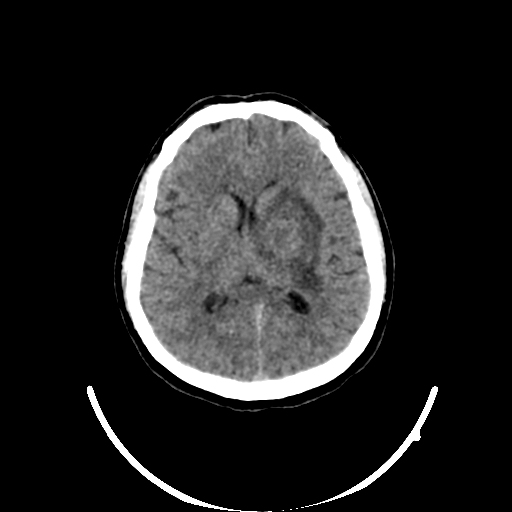
\includegraphics[width=0.7\textwidth]{images/CT-Scan.jpeg}
	\caption{\textit{CT Scan} Otak 
		\autocite{kamesh2024brain}}
	\label{gambar:ctscan}
\end{figure}

\textit{CT Scan} dapat digunakan untuk mengidentifikasi penyakit atau cedera, seperti mencitrakan kepala untuk menemukan cedera, tumor, atau gumpalan yang menyebabkan \textit{stroke} serta mencitrakan paru-paru atau patah tulang yang kompleks. Disamping kelebihan yang dipunyai, \textit{CT Scan} memiliki kelemahan berupa prosedur ini menggunakan radiasi yang memiliki risiko biologis dan agen kontrasnya berpotensi menyebabkan reaksi alergi atau gangguan ginjal pada pasien tertentu \autocite{nibib2022ct}.

\begin{figure}[h]
	\centering
	\captionsetup{justification=centering}
	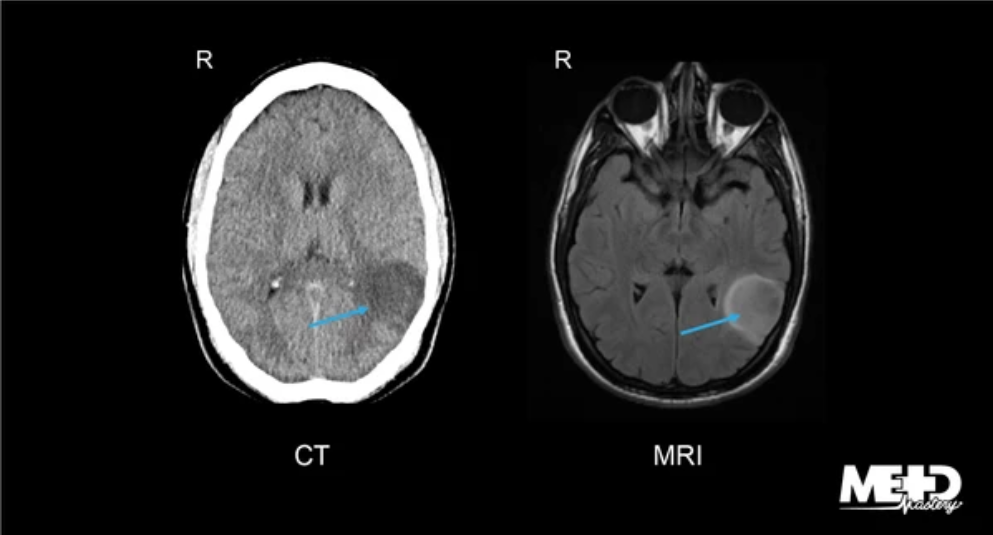
\includegraphics[width=0.7\textwidth]{images/ctvsmri.png}
	\caption{Perbandingan \textit{CT Scan} dan MRI Otak 
		\autocite{mamourian2020recognizing}}
	\label{gambar:ctvsmri}
\end{figure}

Selain risiko biologis, \textit{CT Scan} juga kurang sensitif dalam mendiagnosis, seperti yang terlihat pada Gambar \ref{gambar:ctvsmri}. Pada kasus tumor \textit{intra-axial}, masalah utamanya adalah kurang jelasnya gambar jaringan lunak. Menurut \textcite{mamourian2020recognizing}, banyak tumor jenis ini bersifat \textit{isodense} atau kepadatannya mirip dengan jaringan otak normal. Akibatnya, tumor sulit dibedakan jika tidak memakai cairan kontras atau dibandingkan dengan hasil MRI. Selain itu, sering terjadi kebingungan diagnosis karena tumor bisa terlihat seperti penyakit lain, seperti infark subakut, abses otak, atau lesi demielinisasi. Masalah ini bisa diperparah oleh bias konfirmasi, di mana pembacaan hasil \textit{CT Scan} terpengaruh oleh riwayat penyakit pasien. Oleh karena itu, kunci untuk mendeteksi tumor \textit{intra-axial} pada \textit{CT Scan} adalah dengan mengamati tanda-tanda kecil lainnya secara teliti \autocite{mamourian2020recognizing}.

\section{\textit{Artificial Intelligence} (AI) dalam Pencitraan Medis}
Implementasi AI memberikan dampak besar pada berbagai tugas dalam alur kerja radiologi. AI berdampak pada tugas-tugas klinis berbasis gambar, yang mencakup deteksi kelainan, karakterisasi objek dalam gambar menggunakan segmentasi, diagnosis, dan penentuan stadium, serta pemantauan objek untuk diagnosis dan penilaian respons pengobatan. Terdapat dua metode utama dalam pencitraan medis untuk tugas klasifikasi seperti membedakan tumor jinak atau ganas, yaitu \textit{machine learning} tradisional dan \textit{deep learning} \autocite{hosny2018artificial}.

Dalam konteks transparansi dan kemampuan interpretasi keputusan medis, model-model pembelajaran mesin tersebut dapat dikategorikan lebih lanjut menjadi dua jenis utama \autocite{moreira2024benchmarking}:

\begin{enumerate}
	\item \textit{White-Box Models} \\
	Model ini dirancang dengan logika dasar dan proses yang jelas, sehingga mekanisme pengambilan keputusannya secara dapat ditafsirkan (\textit{interpretable}) oleh manusia. Pengguna dapat memahami bagaimana model bekerja dengan memeriksa struktur internalnya secara langsung, seperti melihat bobot fitur atau aturan keputusan. Contoh algoritma yang termasuk dalam kategori ini adalah \textit{Decision Trees} dan regresi linear.
	
	\item \textit{Black-Box Models} \\
	Model ini memiliki mekanisme internal yang sangat kompleks sehingga sulit atau tidak mungkin bagi pengguna manusia untuk memahami bagaimana prediksi atau hasil spesifik dihasilkan. Karena kompleksitasnya, hubungan antara input dan output sering dianggap sebagai misteri yang tidak dapat diperiksa secara manual. \textit{Deep Neural Networks} dan model \textit{ensemble} yang rumit merupakan representasi utama dari kategori ini.
\end{enumerate}

\subsection{\textit{Machine Learning} Tradisional}
Metode ini bergantung pada \textit{engineered features} yang diekstraksi berdasarkan pengetahuan ahli dari area yang diminati. Contoh fitur ini adalah volume, bentuk, dan tekstur tumor. Fitur-fitur ini kemudian dipilih dan dimasukkan ke alat klasifikasi \autocite{hosny2018artificial}. 

\subsection{\textit{Deep Learning}}
\textit{Deep learning} menggunakan sistem \textit{layers} yang secara bersamaan melakukan ekstraksi fitur, seleksi, dan klasifikasi selama proses pelatihan. Lapisan-lapisan ini belajar mengenali fitur dari yang abstrak, seperti garis hingga yang kompleks, seperti organ \autocite{hosny2018artificial}. Beberapa teknik utama yang biasa digunakan, yaitu:

\begin{enumerate}
	\item CNN (\textit{Convolutional Neural Networks})
	
	CNN adalah model \textit{deep learning} yang dirancang untuk memproses data dengan topologi seperti \textit{grid} dengan contoh berupa gambar. CNN dapat digunakan untuk mendeteksi objek dalam gambar seperti orang, mobil, dan bangunan. CNN juga dapat digunakan untuk melokalisasi objek dalam gambar, yang berarti dapat mengidentifikasi lokasi suatu objek dalam gambar. 
	
	CNN memiliki beberapa komponen kunci. Pertama, \textit{convolutional layers} yang menerapkan filter pada gambar masukan untuk mendeteksi fitur seperti tepi dan tekstur, sekaligus menjaga hubungan spasial antarpiksel. Kedua, \textit{pooling layers} yang melakukan pengurangan sampel untuk mengurangi kompleksitas komputasi dan jumlah parameter. Ketiga, \textit{activation functions} yang memperkenalkan non-linearitas agar model dapat mempelajari hubungan data yang kompleks. Terakhir, \textit{fully connected layers} yang bertanggung jawab membuat prediksi akhir berdasarkan fitur yang telah dipelajari oleh lapisan-lapisan sebelumnya \autocite{gfg2020cnn}. 
	
	\item RNN (\textit{Recurrent Neural Networks}) 
	
	\textit{Recurrent Neural Network} (RNN) adalah \textit{deep neural network} yang dilatih pada data sekuensial untuk menciptakan model \textit{machine learning} yang dapat membuat prediksi atau kesimpulan sekuensial berdasarkan \textit{input} sekuensial \autocite{stryker2021rnn}.  RNN dianggap sangat penting ketika menangani data citra medis yang bersifat sekuensial, seperti video atau gambar \textit{time-series}, karena kemampuannya menangkap ketergantungan waktu \autocite{li2023medical}. 
	
	RNN memiliki dua komponen kunci, yaitu \textit{recurrent neuron} dan RNN \textit{unfolding}. \textit{Recurrent neuron} merupakan unit pemrosesan yang menyimpan keadaan tersembunyi yang berfungsi sebagai memori untuk menyimpan informasi dari \textit{input-input} sebelumnya dalam suatu urutan sehingga memungkinkannya menangkap dependensi antarwaktu. RNN \textit{unfolding} adalah proses struktur rekuren yang direpresentasikan sebagai rangkaian lapisan yang berurutan sesuai langkah waktu. Proses penguraian ini mengilustrasikan aliran informasi dan memungkinkan penerapan algoritma \textit{backpropagation through time}, yaitu metode penyebaran galat mundur melintasi langkah-langkah waktu untuk menyesuaikan bobot jaringan dan mempelajari dependensi dalam data sekuensial \autocite{stryker2021rnn}. 
	
	\item \textit{Generative Adversarial Network} (GAN)
	
	\textit{Generative Adversarial Network} (GAN) adalah model \textit{machine learning} yang dirancang untuk menghasilkan data realistis dengan mempelajari pola dari \textit{dataset} pelatihan yang ada \autocite{varughese2525gan}. GAN memainkan peran penting dalam tugas-tugas yang memerlukan pembuatan atau translasi gambar \autocite{li2023medical}. GAN didasarkan pada dua komponen \textit{neural network}, yaitu generator dan diskriminator. Generator adalah jaringan yang bertugas menghasilkan data sintetis dari \textit{input} acak. Tujuan generator adalah untuk mempelajari pola data asli dan menciptakan sampel palsu. Diskriminator berfungsi sebagai pengklasifikasi biner yang dilatih untuk membedakan antara data nyata dari distribusi data asli dan data palsu yang dihasilkan oleh generator \autocite{gfg2019gan}. 
	
\end{enumerate}

\section{\textit{Explainable AI} (XAI)}
\textit{Explainable Artificial Intelligence} (XAI) adalah seperangkat proses dan metode yang memungkinkan pengguna manusia untuk memahami hasil dan keluaran yang dibuat oleh algoritma \textit{machine learning} \autocite{ibm2023xai}. Tujuan utama \textit{Explainable AI} adalah untuk mendapatkan model yang dapat diinterpretasikan oleh manusia. Interpretasi ini sangat penting untuk aplikasi di sektor-sektor sensitif seperti militer, perbankan, dan layanan kesehatan. Hal ini bertujuan agar para spesialis domain dapat diberikan penjelasan yang bermakna sehingga mereka dapat memahami dan memercayai solusi AI tersebut \autocite{ali2023explainable}.

\subsection{Metode \textit{Explainable AI} (XAI)}
\label{sec:metode_xai}
Berdasarkan mekanisme interpretasi, XAI memiliki hierarki yang dapat dilihat pada Gambar \ref{gambar:hierarkiXAI}.

\begin{figure}[h]
	\centering
	\captionsetup{justification=centering}
	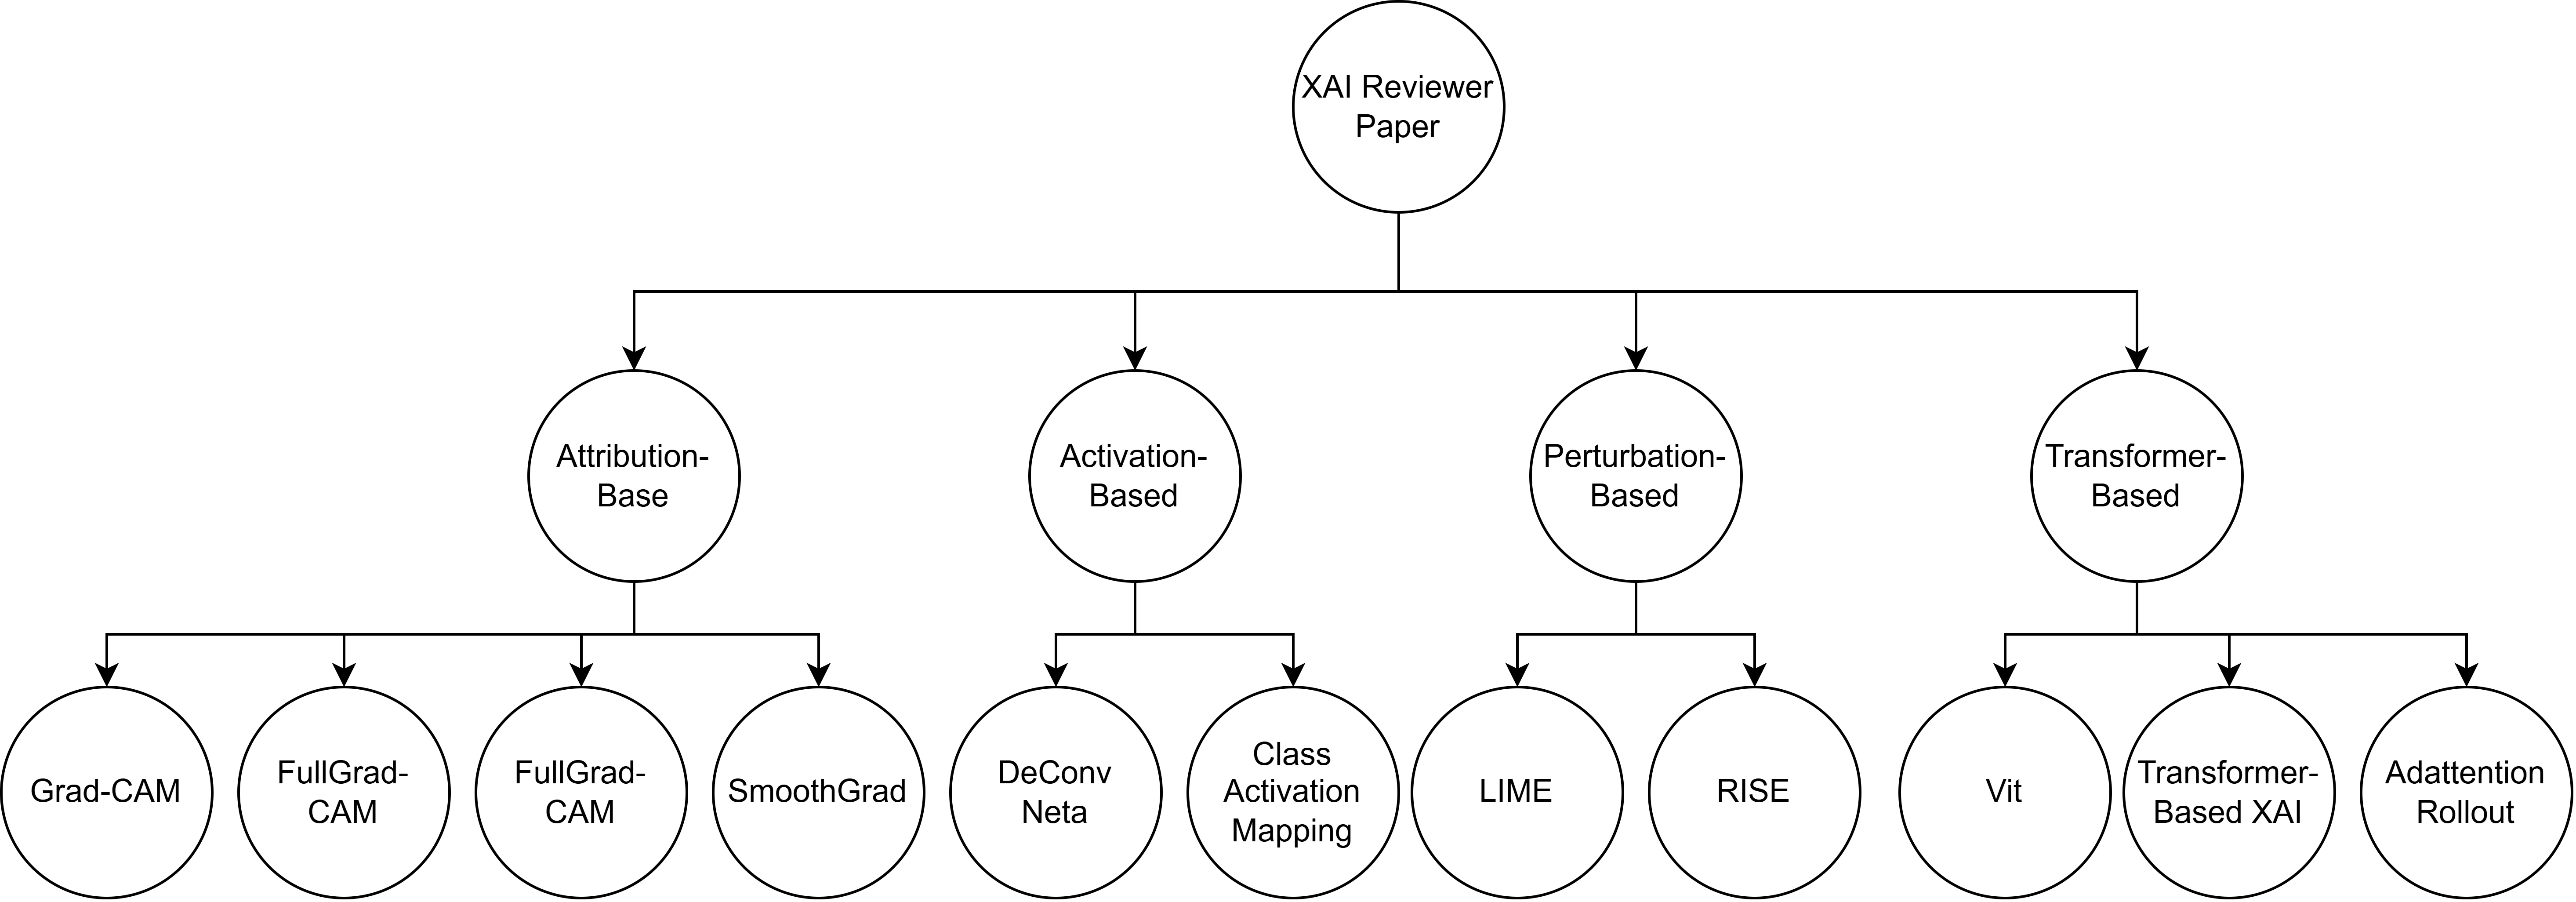
\includegraphics[width=0.7\textwidth]{images/HierarkiXAI.png}
	\caption{Kategorisasi hierarkis metode XAI \autocite{iftikhar2025explainable}}
	\label{gambar:hierarkiXAI}
\end{figure}

\textit{Attribution-based methods} memiliki konsep dengan memberi nilai pada setiap bagian masukan gambar. Bagian yang paling memengaruhi keputusan akhir akan mendapat nilai tinggi. Hal ini dapat membantu penggunanya untuk melihat area pada gambar yang paling penting bagi AI. \textit{Activation-based methods} melihat bagian gambar yang membuatnya bereaksi untuk memberikan penjelasan bagaimana AI mengenali fitur gambar secara bertahap. \textit{Perturbation-based methods} menjelaskan keputusan dengan memodifikasi atau melakukan \textit{masking} sebagian masukan dan mengamati dampaknya pada keluaran. \textit{Transformer-based methods} memanfaatkan mekanisme \textit{self-attention} dari \textit{vision transformers} dan model terkait sehingga bisa menunjukkan bagian gambar yang sedang fokus diperhatikan oleh AI saat mengambil keputusan \autocite{iftikhar2025explainable}.

\subsubsection{\textit{Attribution-based Methods}}
\textit{Attribution-based methods} menghasilkan visualisasi seperti \textit{heatmap} dengan cara melacak representasi \textit{internal model}, seperti gradien atau aktivasi, secara mundur dari \textit{output} prediksi ke \textit{input}. Metode ini memiliki asumsi bahwa tingkat kepentingan sebuah fitur \textit{input} dapat diturunkan dari bagaimana perubahan pada fitur tersebut memengaruhi \textit{output} akhir model. Terdapat beberapa algoritma \textit{attribution-based methods} \autocite{iftikhar2025explainable}, yaitu:

\begin{enumerate}
	\item \textit{Gradient-weighted Class Activation Mapping} (Grad-CAM)\\
	Grad-CAM adalah sebuah metode XAI yang digunakan untuk memahami pentingnya berbagai lapisan dan fitur dalam sebuah CNN. Fungsi utamanya adalah membantu menemukan wilayah pada sebuah gambar yang memiliki dampak terbesar terhadap prediksi model.
	
	\item FullGrad-CAM dan FullGrad-CAM++\\
	Metode FullGrad-CAM dan FullGrad-CAM++ memperluas Grad-CAM dengan menggabungkan semua kontribusi bias dan gradien dari lapisan-lapisan sebelumnya. FullGrad-CAM melakukan \textit{backpropagate gradient} dan mengakumulasi nilai absolutnya untuk menghasilkan penjelasan yang lebih informatif. 
	
	\item SmoothGrad\\
	SmoothGrad mengurangi \textit{visual noise} dengan menambahkan \textit{Gaussian perturbation} kecil ke masukan beberapa kali dan mengambil rata-rata penjelasan berbasis gradien dari variasi-variasi ini. Hal ini dapat menghaluskan perubahan nilai yang sangat drastis yang muncul dalam metode berbasis gradien.
	
\end{enumerate}

\subsubsection{\textit{Perturbation-based Methods}}
\textit{Perturbation-based methods} menjelaskan prediksi model dengan sengaja mengubah \textit{input} dan mengamati bagaimana \textit{output}-nya berubah. Saat sebuah bagian dari \textit{input} ditutupi, diubah, atau dihilangkan dan menyebabkan prediksi model berubah drastis, bagian tersebut akan dianggap penting bagi keputusan model. Terdapat beberapa algoritma \textit{perturbation-based methods} \autocite{iftikhar2025explainable}, yaitu:

\begin{enumerate}
	\item 	LIME (\textit{Local Interpretable Model-Agnostic Explanations})\\
	Metode LIME membagi \textit{input} menjadi segmen-segmen yang dapat ditafsirkan lalu mengganggu segmen-segmen ini dengan menyalakan atau mematikannya secara acak dan melatih model lokal yang lebih sederhana untuk meniru keputusan model \textit{black-box} hanya di area tersebut. Bobot atau tingkat kepentingan dari model ini yang digunakan untuk menjelaskan fitur yang paling penting.
	
	
	\item RISE (\textit{Randomized Input Sampling for Explanation})\\
	Metode RISE bekerja dengan membuat banyak \textit{mask} biner secara acak yang menutupi bagian-bagian gambar. Setiap gambar yang ditutupi \textit{mask} dimasukkan ke model untuk dilihat skor prediksinya. Setelah itu, peta yang menunjukkan bagian penting dihasilkan dengan menggabungkan semua \textit{mask} acak tersebut.
	
\end{enumerate}

\subsubsection{\textit{Activation-based Methods}}
\textit{Activation-based methods} adalah teknik yang menghasilkan penjelasan dengan cara melihat langsung \textit{feature maps} di dalam lapisan-lapisan jaringan saraf (CNN). Terdapat beberapa algoritma \textit{activation-based methods} \autocite{iftikhar2025explainable}, yaitu:


\begin{enumerate}
	\item DeConvNets (\textit{Deconvolutional Networks})\\
	Metode DeConvNets memiliki tujuan untuk memahami dan memvisualisasikan apa yang telah dipelajari oleh setiap neuron atau lapisan dalam sebuah CNN. Metode DeConvNets mengambil sebuah aktivasi fitur dari lapisan dalam seperti neuron yang aktif dan merekonstruksinya kembali ke ruang \textit{input}. Hasil dari metode ini adalah sebuah gambar yang menunjukkan pola visual yang membuat neuron tersebut aktif.
	
	\item \textit{Class Activation Mapping} (CAM)\\
	Metode CAM dilakukan untuk mengidentifikasi wilayah pada gambar \textit{input} yang paling penting yang digunakan model untuk membuat prediksi kelas tertentu. CAM melihat \textit{importance weights} dari lapisan \textit{global average pooling} yang terletak tepat sebelum lapisan keputusan akhir. Setelah itu, CAM menyorot area pada gambar asli yang yang memiliki peta fitur penting aktif. Hasilnya adalah sebuah \textit{heatmap} yang menunjukkan lokasi bukti. 
	
\end{enumerate}

\subsubsection{\textit{Transformer-based Methods}}
\textit{Transformer-based} merupakan metode khusus pada arsitektur \textit{Vision Transformer} (ViT) yang berfokus pada mekanisme \textit{attention} bawaan dari model itu sendiri. ViT memproses gambar dengan membaginya menjadi beberapa potongan dan kemudian menghitung skor atensi di antara semua \textit{patch} tersebut. Teknik ini mengekstrak dan memvisualisasikan skor atensi ini untuk menghasilkan peta yang menunjukkan bagian gambar yang paling diperhatikan oleh model saat mengambil keputusan \autocite{iftikhar2025explainable}.

\section{Evaluasi Model}
Evaluasi model ML sangat penting tidak hanya untuk mengukur kinerja kuantitatif tetapi juga untuk menilai kelayakan praktisnya dalam skenario berisiko tinggi. Evaluasi sangat krusial untuk menyeimbangkan \textit{trade-off} antara akurasi deteksi dengan \textit{false positive rate} untuk mengurangi alarm palsu dan \textit{false negative rate} untuk menghindari ancaman yang terlewat. Selain itu, evaluasi juga mencakup penilaian kualitas dari penjelasan XAI untuk memastikan model tidak hanya akurat tetapi juga transparan, dapat ditafsirkan, dan dapat dipercaya untuk adopsi di dunia nyata \autocite{mohale2025evaluating}.

\subsection{\textit{Deep Learning}}
Salah satu komponen penting dari \textit{deep learning} untuk melatih dan mengevaluasi model adalah \textit{loss function} dan \textit{performance metrics}. \textit{Loss function} mengukur seberapa efektif sebuah model dapat mengaproksimasi keluaran yang diinginkan. Berdasarkan \textcite{terven2025survey}, terdapat beberapa \textit{loss functions} yang bisa digunakan dalam pendeteksian tumor, yaitu:

\begin{enumerate}
	\item \textit{Weighted Cross-Entropy} (WCE) \\
	Memberikan bobot yang lebih tinggi pada kelas minoritas untuk memastikan kelas tersebut mendapat perhatian yang cukup selama pelatihan.
	\item \textit{Dice Loss} \\
	\textit{Loss function} yang umum digunakan dalam pencitraan medis, terutama untuk skenario objek kecil, seperti tumor. \textit{Loss function} ini secara langsung mengoptimalkan tumpang tindih spasial antara prediksi dan target.
	\item \textit{Tversky Loss} \\
	\textit{Tversky Loss} dirancang untuk data dengan \textit{class imbalance} yang parah. \textit{Loss function} ini memungkinkan penalti yang berbeda untuk \textit{false positives} dan \textit{false negatives}, yang sangat penting dalam deteksi medis, seperti melewatkan tumor atau \textit{false negative} memiliki akibat yang lebih fatal.
	
\end{enumerate}

\textit{Performance metrics} menilai kemampuan model untuk membuat prediksi akurat pada data yang belum pernah dilihat. Berdasarkan \textcite{terven2025survey}, terdapat beberapa \textit{performance metrics} yang bisa digunakan dalam pendeteksian tumor, yaitu:

\begin{enumerate}
	\item \textit{Precision}, \textit{Recall}, dan \textit{F1-Score} \\
	\textit{Precision} mengukur akurasi prediksi positif, \textit{recall} mengukur seberapa banyak kasus tumor aktual yang berhasil ditemukan, dan \textit{F1-Score} memberikan skor keseimbangan antara keduanya.
	\item \textit{Precision-Recall Curve} \\
	Kurva yang memvisualisasikan \textit{trade-off} antara \textit{precision} dan \textit{recall} di berbagai ambang batas. \textit{Precision-recall curve} direkomendasikan untuk data yang tidak seimbang dengan kelas minoritas yang penting.
\end{enumerate}

\subsection{\textit{Explainable Artificial Intelligence} (XAI)}
Berdasarkan \textcite{kadir2023evaluation}, untuk melakukan evaluasi terhadap XAI, diperlukan metrik XAI yang bisa ditentukan oleh dua taksonomi, yaitu taksonomi berbasis aplikasi dan taksonomi berbasis metodologi evaluasi.

\begin{enumerate}
	\item Taksonomi Berbasis Aplikasi \\
	Taksonomi berbasis aplikasi adalah klasifikasi yang mengelompokkan metrik XAI berdasarkan tujuan konseptualnya. Hal ini memisahkan konsep umum seperti \textit{user satisfaction} dan \textit{transparency} dari metode \textit{local explanation} yang lebih teknis beserta turunannya seperti \textit{attribution} dan \textit{saliency} \autocite{kadir2023evaluation}.
	
	\begin{figure}[h]
		\centering
		\captionsetup{justification=centering}
		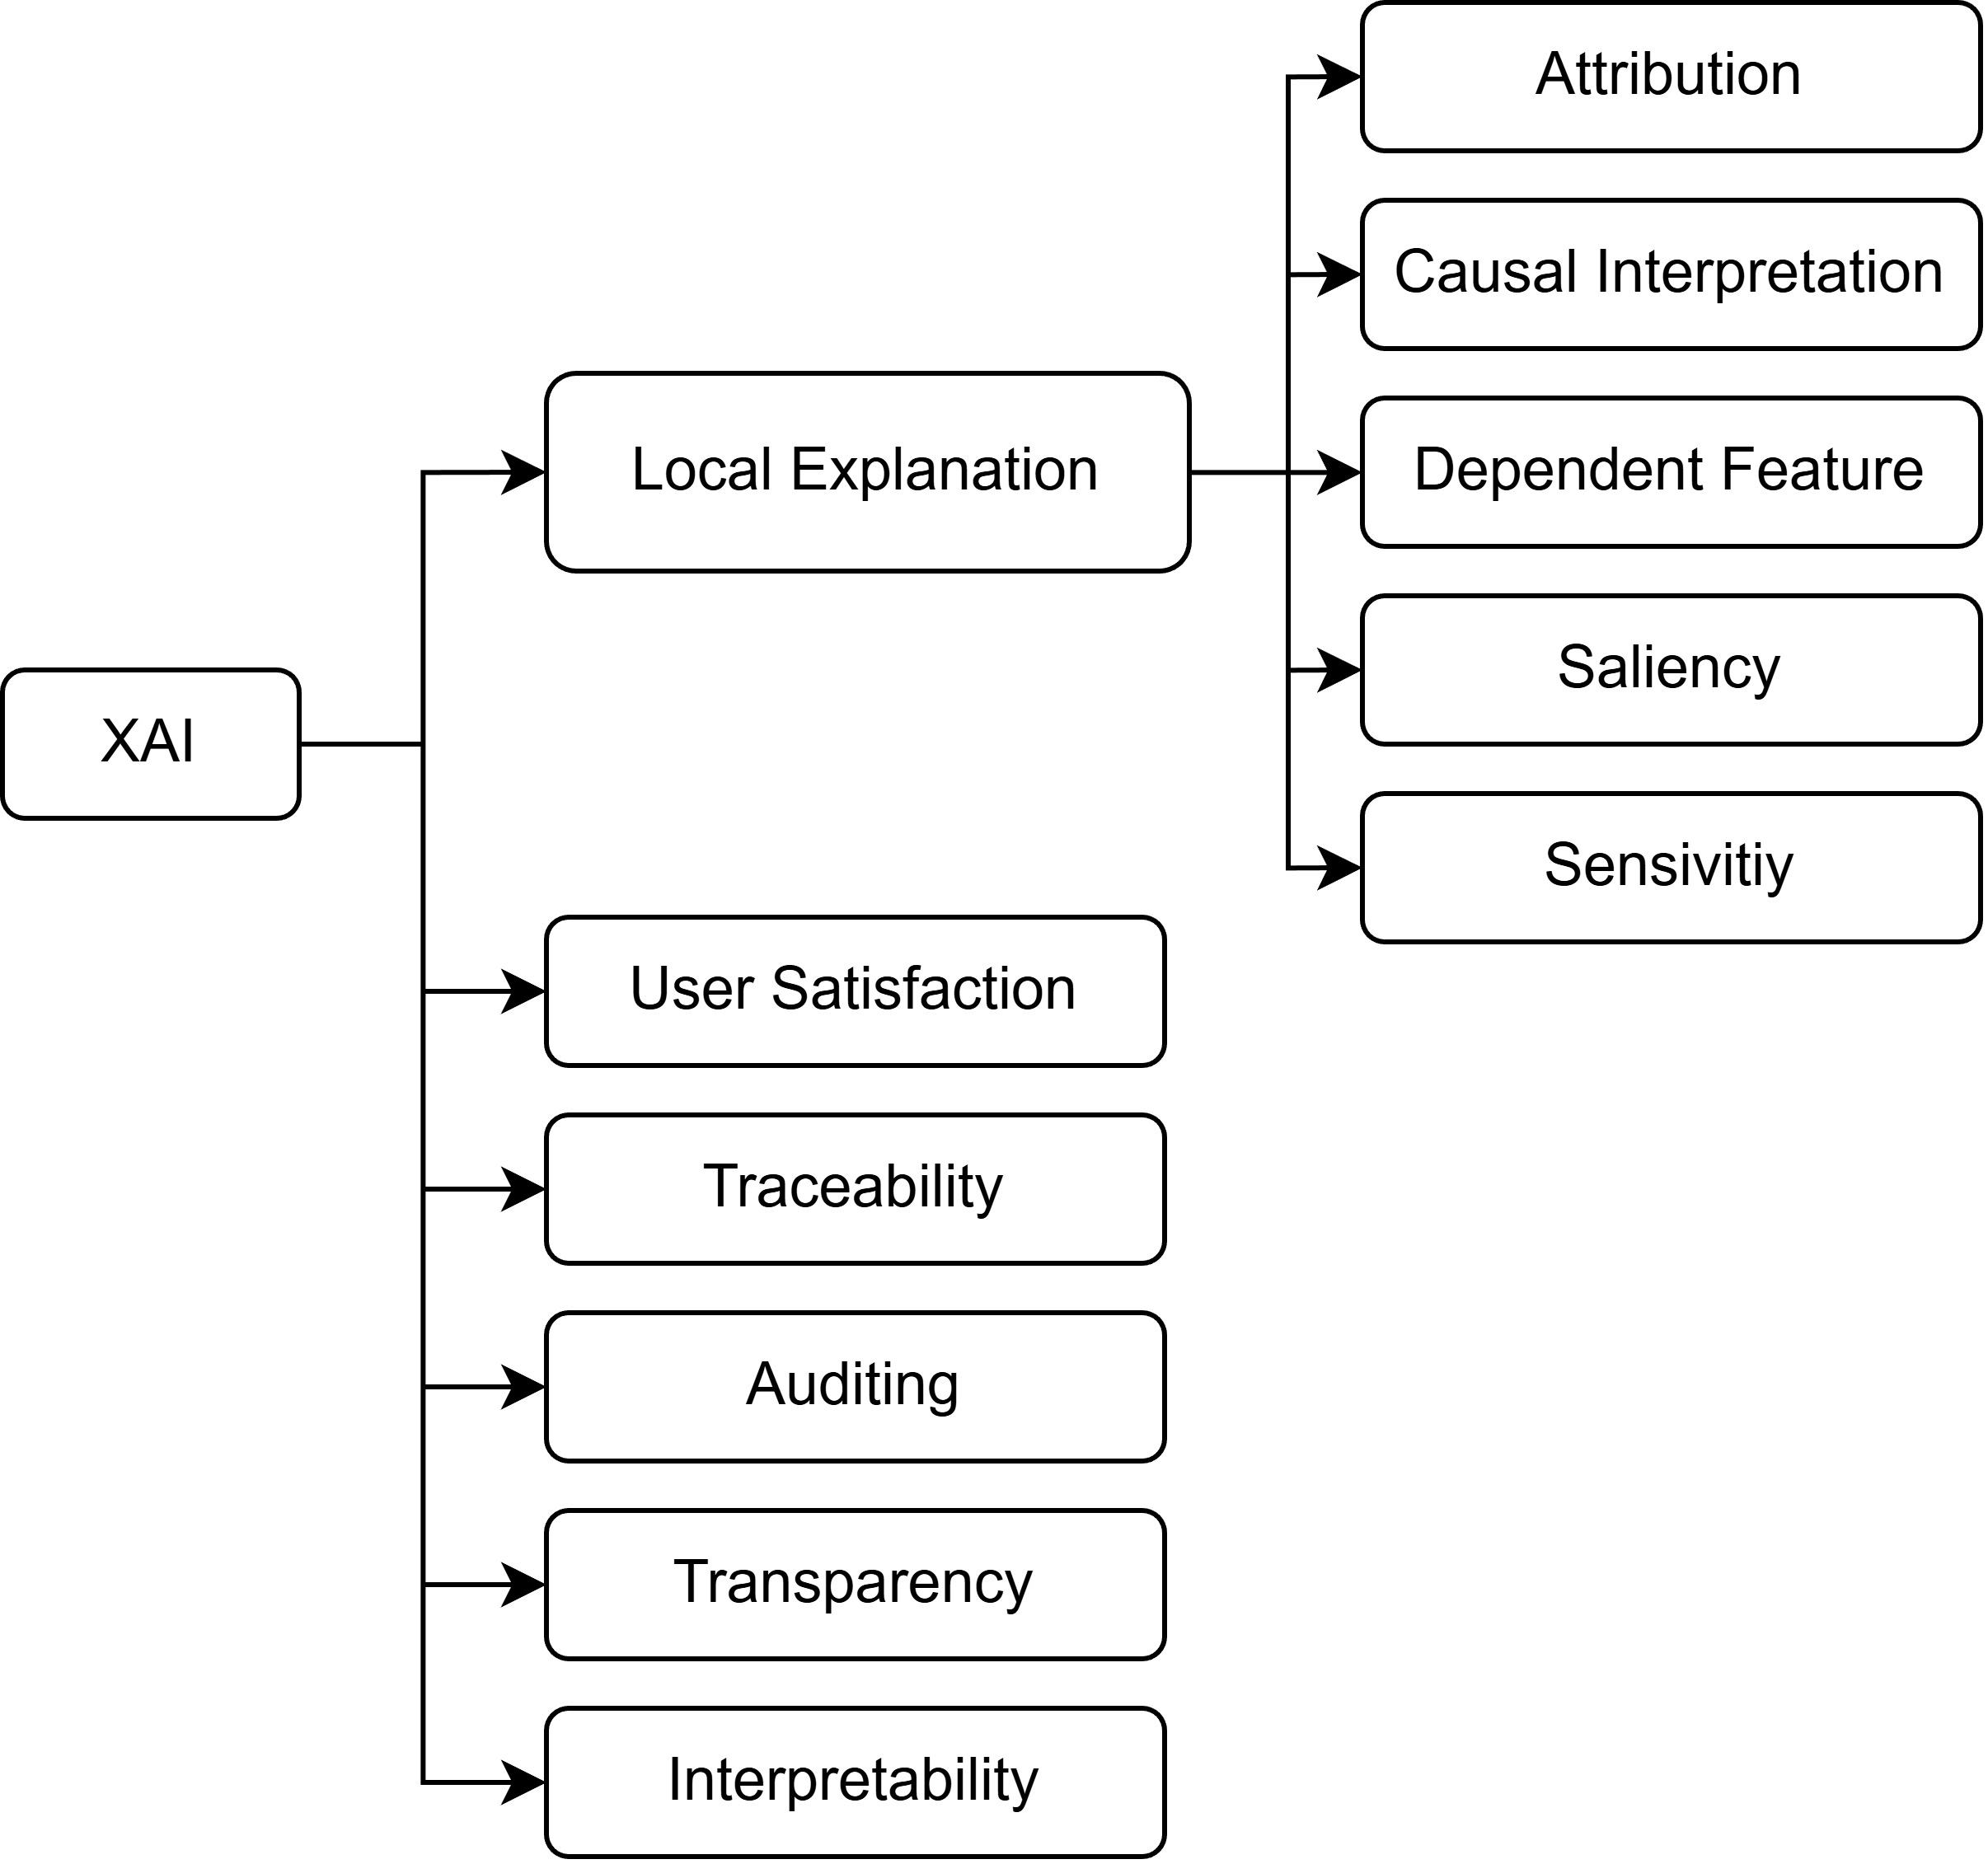
\includegraphics[width=0.7\textwidth]{images/TaksonomiXAI.png}
		\caption{Taksonomi berdasarkan aplikasi XAI \autocite{kadir2023evaluation}}
		\label{gambar:taksonomiXAI}
	\end{figure}
	
	\item Taksonomi Berbasis Metodologi Evaluasi \\
	Taksonomi berbasis metodologi evaluasi mengklasifikasikan teknik-teknik evaluasi penjelasan lokal ke dalam tiga pendekatan teknis utama, yaitu \textit{retraining}, \textit{ground truth comparison}, dan \textit{input perturbation} \autocite{kadir2023evaluation}. 
	
	\begin{figure}[h]
		\centering
		\captionsetup{justification=centering}
		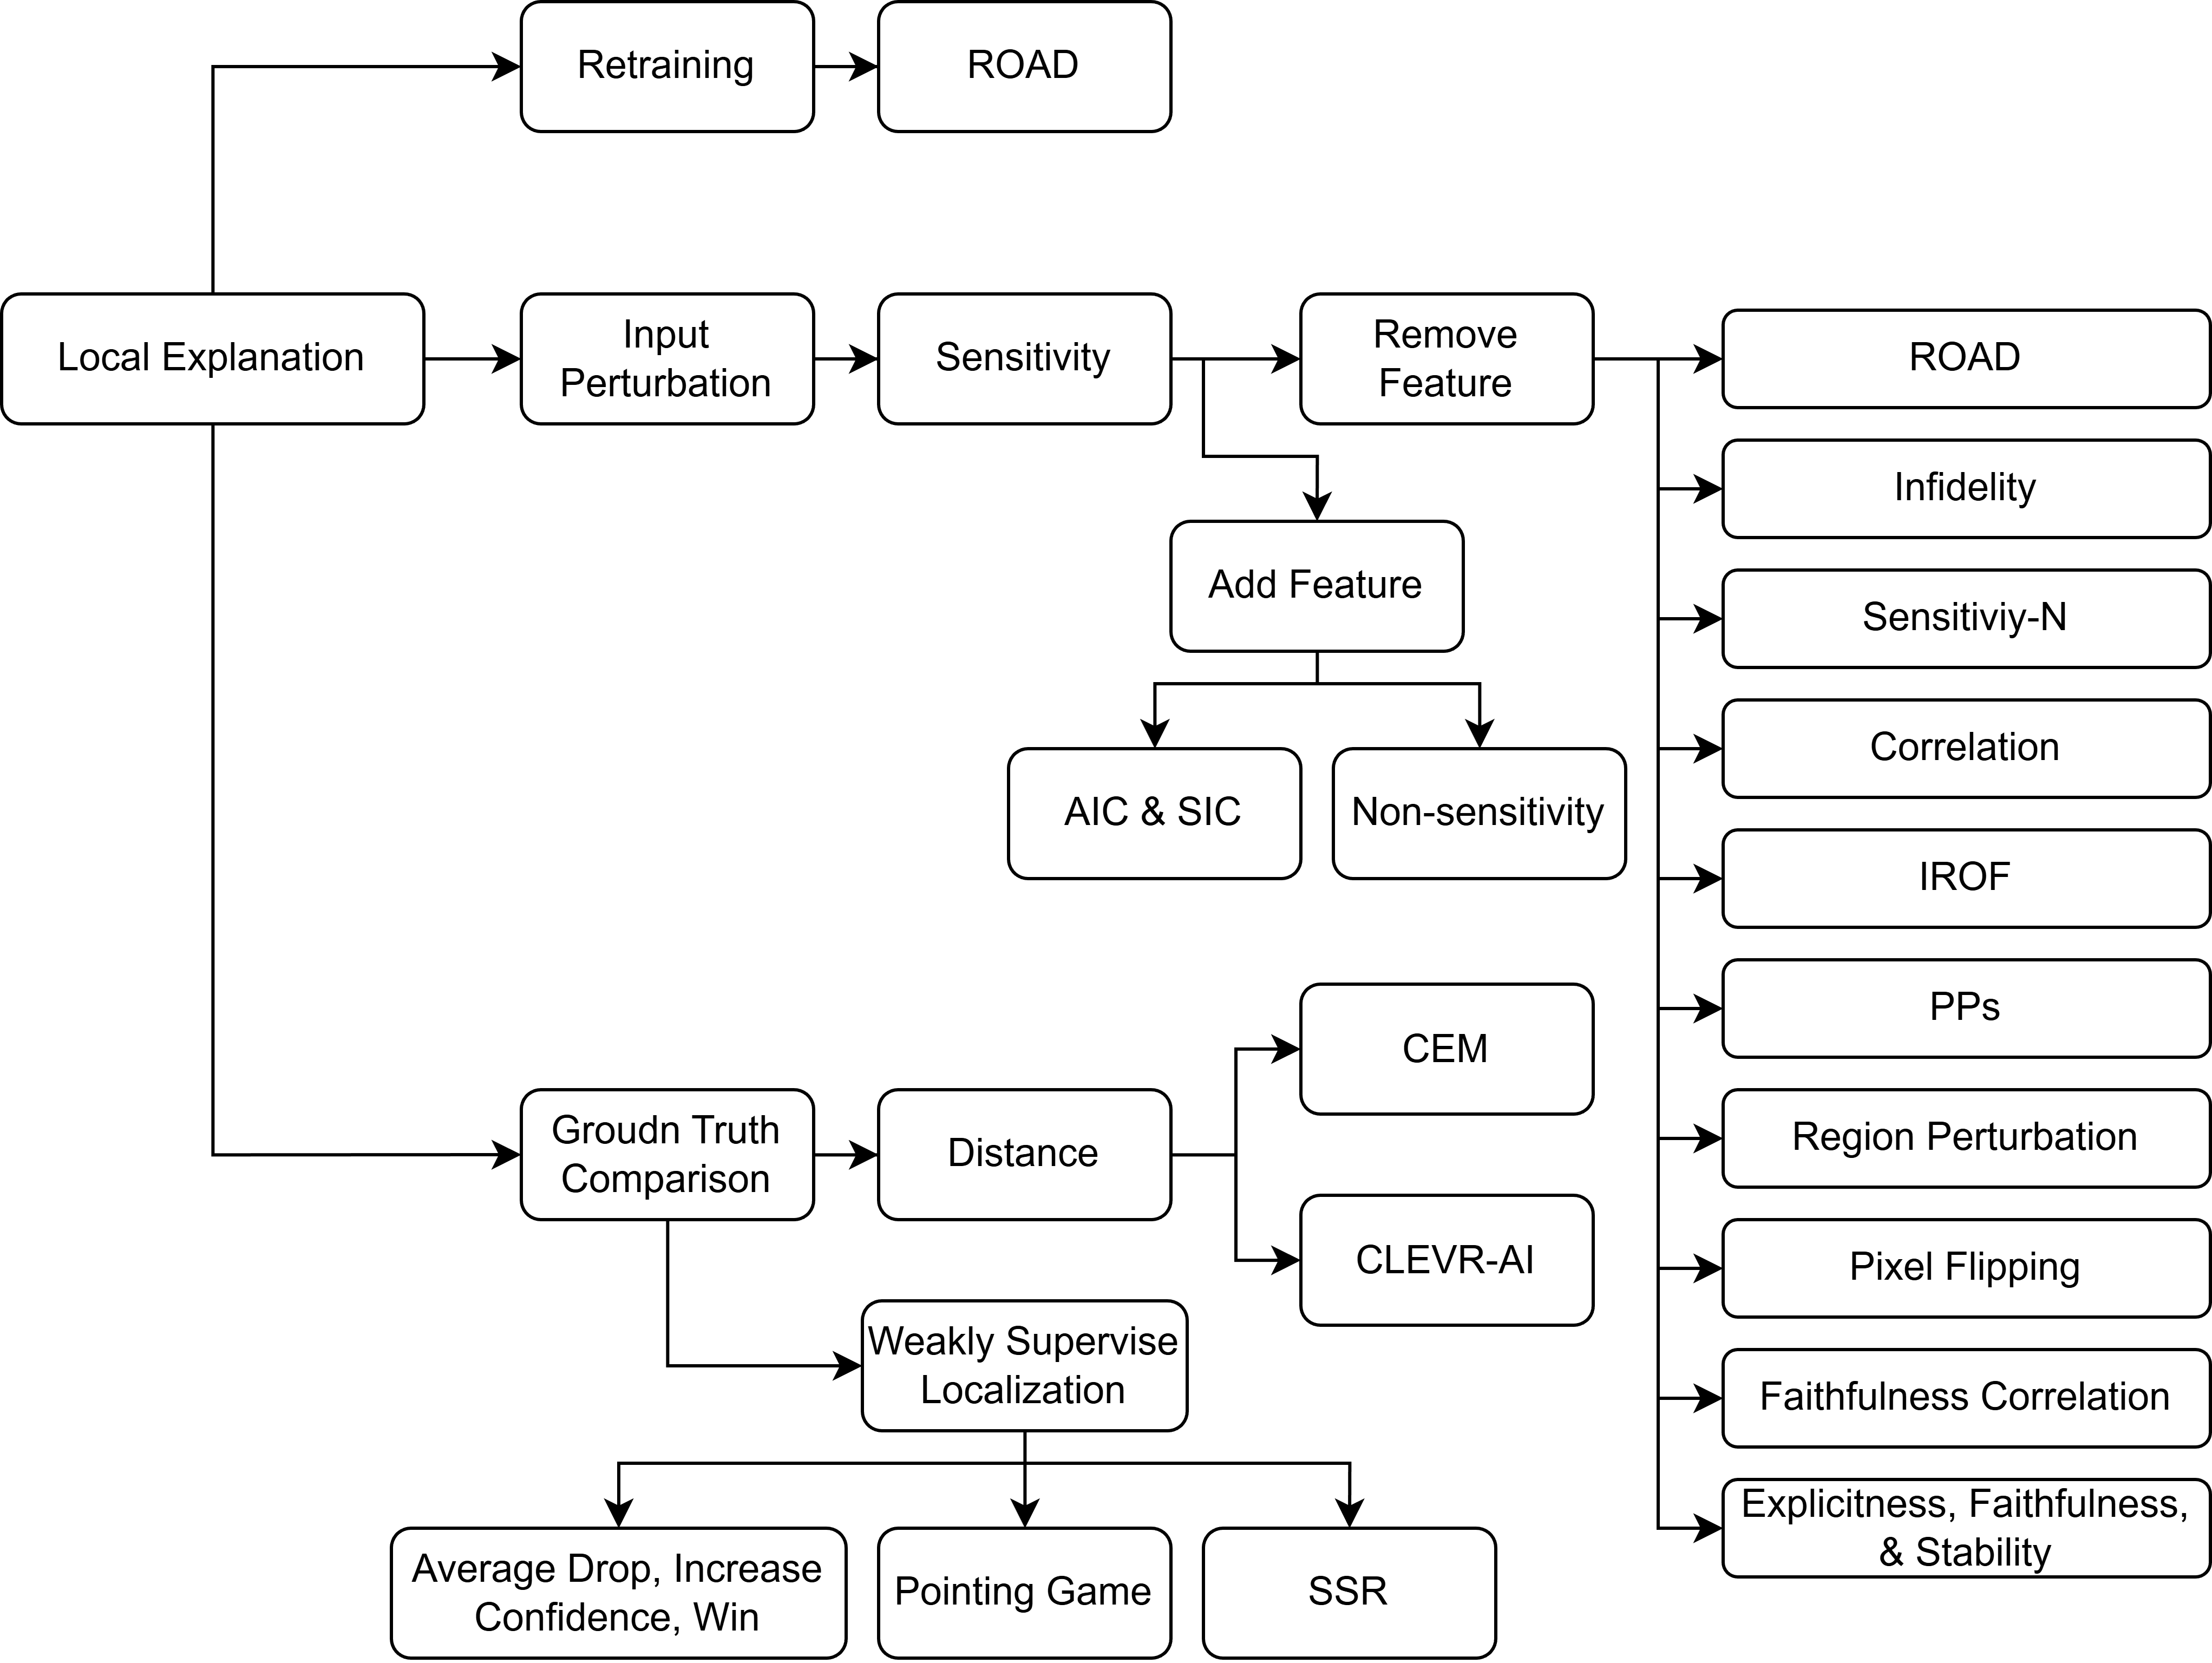
\includegraphics[width=0.7\textwidth]{images/TaksonomiXAI2.png}
		\caption{Taksonomi berdasarkan metodologi evaluasi \autocite{kadir2023evaluation}}
		\label{gambar:taksonomiXAI2}
	\end{figure}
	
	Dalam pendekatan \textit{ground truth comparison}, terdapat penelitian terbaru oleh \textcite{muhammad2025heatmap} yang mengusulkan metrik evaluasi kuantitatif bernama XAlign. Metrik ini dirancang untuk mengatasi keterbatasan metrik yang tumpang tindih standar dengan menilai \textit{spatial fidelity heatmap} melalui tiga komponen integratif yang diformulasikan sebagai berikut.
	
	\begin{enumerate}
		\item \textit{Weighted Relevance Overlap} (WRO) \\
		Komponen ini mengukur proporsi relevansi penjelasan yang terlokalisasi secara tepat di dalam area anotasi ahli. Semakin tinggi nilai WRO, semakin fokus penjelasan tersebut pada area klinis yang relevan. Secara matematis, WRO didefinisikan seperti pada Persamaan \ref{eq:wro}:
		\begin{equation}
			WRO = \frac{\sum_{i \in G} X_{i}}{\sum_{i} X_{i}}
			\label{eq:wro}
		\end{equation}
		$G$ merepresentasikan himpunan piksel dalam masker \textit{ground truth}. $X_i$ adalah skor relevansi intensitas \textit{heatmap} pada piksel ke-$i$.
		
		\item \textit{Boundary Agreement Score} (BAS) \\
		BAS menilai ketepatan penyelarasan struktural antara batas \textit{heatmap} dengan kontur lesi atau tumor menggunakan \textit{Hausdorff Distance} yang dinormalisasi, seperti yang ditunjukkan pada Persamaan \ref{eq:bas}:
		\begin{equation}
			BAS = 1 - \frac{HD(G, X)}{\text{max\_dim}(I)}
			\label{eq:bas}
		\end{equation}
		$HD(G, X)$ adalah jarak Hausdorff antara kontur \textit{ground truth} ($G$) dan peta penjelasan ($X$). $max\_dim(I)$ adalah dimensi maksimum citra untuk normalisasi. Nilai BAS yang mendekati 1 mengindikasikan korespondensi anatomis yang presisi.
		
		\item \textit{Dispersion Penalty} (DP) \\
		Komponen ini memberikan penalti terhadap penyebaran atribusi di luar area klinis untuk memastikan peta \textit{saliency} tetap ringkas, dengan formulasi pada Persamaan \ref{eq:dp}:
		\begin{equation}
			DP = \frac{\sum_{i \notin G} X_{i}}{\sum_{i} X_{i}}
			\label{eq:dp}
		\end{equation}
		$i \notin G$ menunjukkan piksel yang berada di luar area \textit{ground truth}. Nilai DP yang lebih rendah menandakan penjelasan yang lebih fokus dengan sedikit \textit{noise} latar belakang.\\
	\end{enumerate}
	
	Secara keseluruhan, skor akhir XAlign dihitung dengan menggabungkan ketiga komponen tersebut menggunakan bobot skalar ($\alpha, \beta, \gamma$) seperti pada Persamaan \ref{eq:xalign}:
	\begin{equation}
		XAlign = \alpha \cdot WRO + \beta \cdot BAS - \gamma \cdot DP
		\label{eq:xalign}
	\end{equation}
	Penggunaan XAlign memungkinkan evaluasi yang tidak hanya mengukur akurasi lokasi, tetapi juga kepatuhan bentuk penjelasan terhadap anatomi tumor yang sebenarnya \autocite{muhammad2025heatmap}.
\end{enumerate}

Untuk menentukan metrik evaluasi XAI, prosesnya dimulai dengan mengidentifikasi konsep yang akan diuji menggunakan taksonomi berbasis aplikasi. Taksonomi ini membantu membedakan apakah tujuannya adalah untuk mengukur konsep umum seperti \textit{user satisfaction} dan \textit{transparency}, atau untuk mengevaluasi penjelasan teknis yang lebih spesifik seperti \textit{local explanation}, yang mencakup metode seperti \textit{saliency}. Setelah itu, taksonomi berbasis metodologi evaluasi digunakan untuk memilih pendekatan teknis yang sesuai untuk mengevaluasi penjelasan lokal tersebut \autocite{kadir2023evaluation}.

\section{Penelitian Terkait}
\subsection{\textit{Explainable CNN for brain tumor detection and classification through XAI based key features identification}}
Penelitian terbaru yang dilakukan oleh \textcite{Iftikhar2025ExplainableCNN} mengajukan pendekatan \textit{explainable} CNN untuk klasifikasi tumor otak guna mengatasi sifat \textit{black-box} pada model \textit{deep learning} yang sering kali menghambat transparansi klinis. Penelitian ini menyoroti bahwa kompleksitas struktur model yang berlebihan sering kali menyebabkan model bergantung pada fitur yang tidak relevan, seperti jaringan lunak normal, yang menurunkan kepercayaan terhadap hasil diagnosis. Untuk mengatasi hal tersebut, \textcite{Iftikhar2025ExplainableCNN} mengembangkan metodologi yang mengintegrasikan teknik \textit{Explainable AI} (XAI), khususnya \textit{Gradient-weighted Class Activation Mapping} (Grad-CAM), \textit{Shapley Additive Explanations} (SHAP), dan \textit{Local Interpretable Model-agnostic Explanations} (LIME) ke dalam arsitektur CNN. Inovasi utama dalam penelitian ini adalah pemanfaatan analisis Grad-CAM untuk menyederhanakan arsitektur model dengan memangkas \textit{layer} yang memiliki kontribusi minimal terhadap keputusan prediksi sehingga menghasilkan model yang lebih efisien tanpa mengorbankan akurasi.

Evaluasi performa dilakukan menggunakan \textit{dataset} MRI publik dengan empat kelas klasifikasi, yaitu \textit{meningioma}, \textit{glioma}, \textit{pituitary}, dan \textit{no tumor}. Hasil penelitian menunjukkan bahwa model berbasis XAI yang diusulkan mampu mencapai akurasi sebesar 99,21\% pada \textit{dataset} latih dan 94,72\% pada data uji yang belum pernah dilihat. Evaluasi juga menunjukkan keseimbangan yang baik antara presisi dan \textit{recall}. Secara kualitatif, visualisasi XAI membuktikan bahwa model mampu memfokuskan perhatian pada area patologis yang spesifik berbeda dengan model awal tanpa XAI yang perhatiannya sering tersebar ke area tanpa tumor.

Studi dari \textcite{Iftikhar2025ExplainableCNN} memiliki keterbatasan karena hanya berfokus pada modalitas pencitraan MRI yang saat ini menjadi permasalahan di Indonesia. Para peneliti secara eksplisit menyarankan penelitian masa depan untuk menguji efektivitas metode serupa pada modalitas lain, seperti \textit{CT Scan} untuk memperluas jangkauan diagnostik. Celah penelitian menjadi salah satu landasan bagi tugas akhir ini untuk menerapkan integrasi XAI pada citra \textit{CT Scan}, yang memiliki tantangan karakteristik citra berbeda dibandingkan MRI untuk menyediakan solusi diagnostik yang terpercaya di fasilitas kesehatan dengan keterbatasan alat MRI.

\subsection{\textit{Enhanced Classification of Brain MRI Images for Tumor Detection Using Transfer Learning and Grad-CAM-Based Explainable CNN}}

Penelitian yang dilakukan oleh \textcite{putra2025enhanced} mengusulkan kerangka kerja \textit{deep learning} yang menggabungkan \textit{transfer learning} dari model EfficientNet-B0 dengan metode \textit{Explainable AI} (XAI) berbasis Grad-CAM untuk klasifikasi dan deteksi tumor otak. Penelitian ini secara khusus menyoroti pentingnya tahapan \textit{preprocessing} yang dioptimalkan untuk meningkatkan kualitas representasi visual citra masukan sebelum proses ekstraksi fitur dilakukan. Rangkaian \textit{preprocessing} yang diimplementasikan meliputi pengubahan ukuran citra (\textit{resizing}) menjadi 224x224 piksel untuk menyesuaikan dengan arsitektur dasar EfficientNet-B0, serta normalisasi nilai intensitas piksel ke rentang [0,1] guna menstabilkan pembaruan gradien selama proses pelatihan. Sebagai langkah optimasi utama, teknik \textit{Contrast Limited Adaptive Histogram Equalization} (CLAHE) diterapkan untuk meningkatkan kontras lokal dan mempertegas batas-batas tumor, yang dikombinasikan dengan \textit{Gaussian filtering} untuk meredam derau (\textit{denoising}) frekuensi tinggi pada tekstur MRI. Pendekatan ini selanjutnya diperkuat oleh augmentasi data secara probabilistik, seperti rotasi, \textit{flipping}, \textit{zooming}, dan variasi kecerahan, yang secara signifikan memperluas keberagaman \textit{dataset} latih untuk mencegah terjadinya \textit{overfitting}.

Evaluasi performa dilakukan menggunakan \textit{dataset} MRI publik yang terdiri dari 3.000 citra dengan empat kelas kategori: \textit{glioma}, \textit{meningioma}, \textit{pituitary}, dan \textit{no tumor}. Hasil eksperimen membuktikan bahwa integrasi alur \textit{preprocessing} tersebut dengan EfficientNet-B0 mampu mencapai tingkat akurasi sebesar 94,2\% dan nilai AUC 0,965, yang secara signifikan mengungguli model CNN \textit{baseline}. Dari segi transparansi pengambilan keputusan, penggunaan visualisasi Grad-CAM mengonfirmasi bahwa model mampu memfokuskan atensinya (ditunjukkan dengan \textit{heatmap} berintensitas tinggi) pada area lesi tumor secara tepat tanpa mengandalkan artefak latar belakang yang tidak relevan secara klinis.

Meskipun model dari \textcite{putra2025enhanced} mencapai tingkat akurasi dan interpretabilitas yang tinggi, pengujian masih terbatas pada ruang lingkup citra MRI 2D independen dan masih dihadapkan pada tantangan variasi perangkat antar-institusi medis. Ketergantungan eksklusif pada modalitas MRI ini memvalidasi urgensi dan celah penelitian yang diangkat dalam tugas akhir ini, yaitu perancangan sistem pendukung keputusan deteksi tumor otak berbasis XAI yang diterapkan pada citra \textit{CT Scan}. Eksplorasi pada data \textit{CT Scan} akan mengevaluasi seberapa efektif metode \textit{preprocessing} (seperti CLAHE dan reduksi derau) serta ekstraksi fitur visual beradaptasi dengan profil intensitas jaringan yang berbeda pada \textit{CT Scan}, guna memperluas dan menyediakan alternatif diagnosis otomatis yang dapat dipercaya untuk mengatasi keterbatasan aksesibilitas alat MRI di berbagai fasilitas kesehatan.

\subsection{\textit{Performance Evaluation of Preprocessing Techniques for Noise Reduction and Enhancement in MRI-based Brain Tumor Detection}}
Penelitian yang dilakukan oleh \textcite{flower2025performance} mengevaluasi efektivitas berbagai metode pra-pemrosesan yang secara khusus dirancang untuk meningkatkan kualitas citra medis, khususnya MRI, dalam mendeteksi tumor otak. Studi ini menyoroti bahwa citra mentah (\textit{raw images}) sering kali mengalami degradasi kualitas akibat derau (\textit{noise}), tingkat kontras yang rendah, serta keberadaan artefak. Gangguan-gangguan tersebut dapat menyulitkan proses interpretasi dan menurunkan keandalan algoritma deteksi maupun segmentasi. Untuk mengatasi tantangan tersebut, penelitian ini membandingkan teknik reduksi derau, yang meliputi filter \textit{Gaussian}, \textit{median}, \textit{Non-Local Means} (NLM), dan \textit{wavelet}, dengan teknik peningkatan kualitas citra (\textit{image enhancement}), yaitu \textit{Histogram Equalization} (HE), \textit{Contrast Limited Adaptive Histogram Equalization} (CLAHE), dan normalisasi intensitas.

Evaluasi performa dari teknik-teknik pra-pemrosesan ini diukur menggunakan \textit{dataset} publik yang mencakup empat kelas diagnosis: \textit{glioma}, \textit{meningioma}, \textit{pituitary tumor}, dan \textit{no-tumor}. Penilaian dilakukan secara kuantitatif bersandar pada metrik \textit{Mean Squared Error} (MSE), \textit{Peak Signal-to-Noise Ratio} (PSNR), \textit{Structural Similarity Index} (SSIM), dan \textit{Noise Power Spectrum} (NPS). Hasil analisis membuktikan bahwa filter \textit{wavelet} adalah metode paling unggul untuk mereduksi derau, karena teknik dekomposisi frekuensinya mampu menghilangkan derau sambil tetap mempertahankan struktur dan tepi (\textit{edges}) area tumor secara optimal. Di sisi peningkatan kualitas, normalisasi intensitas terbukti superior karena mampu menstandarkan rentang intensitas piksel di seluruh \textit{dataset}, sehingga mengurangi variabilitas yang diakibatkan oleh pengaturan pemindai (\textit{scanner}) yang berbeda-beda. Kombinasi dari filter \textit{wavelet} dan normalisasi intensitas disimpulkan sebagai \textit{pipeline} pra-pemrosesan yang paling optimal untuk menghasilkan citra yang konsisten dan berkualitas tinggi.

Meskipun kajian dari \textcite{flower2025performance} diimplementasikan pada modalitas MRI, prinsip rancangan \textit{pipeline} pra-pemrosesan ini dapat diekstrapolasi untuk modalitas pencitraan lain seperti \textit{CT Scan}. Menerapkan teknik reduksi derau yang mampu menjaga detail anatomis dipadukan dengan standardisasi intensitas sangat esensial untuk menyiapkan citra \textit{CT Scan} sebelum masuk ke tahap analisis lebih lanjut. Pendekatan pra-pemrosesan yang komprehensif ini menjadi fondasi krusial ketika mengintegrasikan metode \textit{Explainable AI} (XAI) ke dalam sistem pendukung keputusan. Dengan citra masukan yang bersih dan terstandarisasi, metode visualisasi seperti \textit{Grad-CAM} dapat lebih akurat dalam menyoroti fitur patologis yang sebenarnya dari tumor otak, tanpa terdistraksi oleh artefak maupun inkonsistensi kontras visual.

\subsection{\textit{CT to MRI Image Translation Using CycleGAN: A Deep Learning Approach for Cross-Modality Medical Imaging}}

Dalam upaya menjembatani keterbatasan modalitas pencitraan medis, \textcite{Jha2024CTtoMRI} melakukan penelitian yang berfokus pada translasi citra \textit{CT Scan} menjadi citra yang menyerupai \textit{Magnetic Resonance Imaging} (MRI). Penelitian ini dilatarbelakangi oleh paradoks bahwa MRI menawarkan kontras jaringan lunak yang sangat baik namun proses pemindaiannya lambat dan mahal, sedangkan \textit{CT Scan} jauh lebih cepat namun melibatkan paparan radiasi pengion. Oleh karena itu, penelitian ini bertujuan mengembangkan model \textit{deep learning} menggunakan arsitektur CycleGAN untuk men-translasi \textit{CT Scan} menjadi citra menyerupai MRI. Pendekatan ini diharapkan dapat menghilangkan kebutuhan biaya tambahan dan paparan radiasi ganda bagi pasien.

Metodologi yang diterapkan melibatkan penggunaan \textit{dataset} citra potongan lintang otak untuk CT dan MRI yang tidak berpasangan (\textit{unpaired}). Pemrosesan awal data mencakup penyesuaian dimensi citra menjadi $256 \times 256$ piksel, penskalaan nilai piksel ke rentang [-1, 1], serta penerapan augmentasi data untuk menekan risiko \textit{overfitting}. Inovasi utama dalam arsitektur studi ini adalah pemanfaatan \textit{cycle consistency loss} pada CycleGAN, yang memastikan citra dapat ditranslasi antar domain dan dikembalikan ke bentuk aslinya tanpa kehilangan fidelitas anatomis. Proses ini didukung oleh komponen generator yang terdiri dari \textit{Encoder-Transformer-Decoder} dan diskriminator berbasis arsitektur \textit{PatchGAN}.

Hasil penelitian menunjukkan bahwa model CycleGAN yang diusulkan sangat efektif, mencapai nilai evaluasi \textit{Mean Absolute Error} (MAE) sebesar 0,5309, \textit{Mean Squared Error} (MSE) 0,37901, dan \textit{Peak Signal-to-Noise Ratio} (PSNR) 52,344. Angka-angka ini secara signifikan melampaui performa model CNN dasar (\textit{baseline}) yang kesulitan menangani \textit{dataset} tidak berpasangan. Secara kualitatif, citra MRI sintetik yang dihasilkan terbukti mampu merepresentasikan anatomi otak secara keseluruhan dengan baik, mencakup visualisasi yang jelas pada materi abu-abu, materi putih, cairan serebrospinal, hingga pembuluh darah utama. Meskipun demikian, para peneliti memberikan catatan penting bahwa citra sintetik ini masih kehilangan beberapa detail presisi sehingga belum dapat digunakan secara mentah untuk diagnosis klinis tanpa pertimbangan matang.

Studi ini memberikan landasan teknis yang sangat relevan untuk mengeksplorasi translasi citra lintas modalitas sebagai tahapan pra-pemrosesan diagnostik. Keberhasilan \textcite{Jha2024CTtoMRI} dalam menyintesis citra MRI dari \textit{CT Scan} otak secara khusus mendukung gagasan bahwa mengubah set data \textit{CT Scan} menjadi MRI sintetik berpotensi mengatasi keterbatasan kontras jaringan lunak pada citra aslinya. Pendekatan ini selaras dengan upaya deteksi tumor otak, di mana pengintegrasian teknik \textit{Explainable AI} seperti Grad-CAM ke dalam citra sintetik dengan visibilitas struktur jaringan yang lebih baik diestimasi mampu menghasilkan visualisasi (\textit{heatmap}) penentuan keputusan model yang jauh lebih representatif. Peningkatan kualitas representasi batas anatomis pada tahap pra-pemrosesan ini diharapkan dapat mempermudah model identifikasi dalam menyorot pola abnormal akibat tumor secara lebih transparan dan efisien.

\subsection{\textit{Explainable AI for lung cancer detection via a custom CNN on CT images}}
Dalam upaya mengatasi tantangan diagnosis medis berbasis kecerdasan buatan yang sering kali bersifat \textit{black-box}, \textcite{Hammad2025ExplainableAI} melakukan penelitian yang berfokus pada deteksi kanker paru menggunakan citra \textit{CT Scan}. Penelitian ini dilatarbelakangi oleh permasalahan bahwa analisis manual citra CT memakan waktu dan rentan kesalahan, sementara model \textit{deep learning} sering kali gagal memberikan alasan di balik keputusan prediksi mereka sehingga mengurangi kepercayaan tenaga medis. Oleh karena itu, penelitian ini bertujuan mengembangkan sebuah model \textit{custom Convolutional Neural Network} (CNN) yang tidak hanya memiliki akurasi tinggi, tetapi juga dilengkapi dengan fitur transparansi melalui integrasi teknik \textit{Explainable AI} (XAI).

Metodologi yang diterapkan melibatkan penggunaan \textit{dataset} citra \textit{CT Scan} yang melalui proses pra-pemrosesan dan augmentasi data untuk meningkatkan generalisasi model. Inovasi utama dalam studi ini adalah penerapan metode \textit{Gradient-weighted Class Activation Mapping} (Grad-CAM) untuk menghasilkan \textit{heatmap} visual. Visualisasi ini berfungsi untuk menyoroti area spesifik pada citra CT yang dianggap penting oleh model dalam menentukan klasifikasi sehingga dokter dapat memverifikasi apakah model berfokus pada fitur patologis yang relevan atau sekadar \textit{noise}.

Hasil penelitian menunjukkan bahwa model yang diusulkan mampu mencapai akurasi keseluruhan sebesar 93,06\% dengan presisi dan \textit{recall} yang seimbang di berbagai kelas klasifikasi. Secara kualitatif, hasil visualisasi Grad-CAM mendemonstrasikan bahwa model secara akurat memusatkan perhatian pada batas tumor dan struktur jaringan abnormal, yang selaras dengan diagnosis klinis. Temuan ini mengonfirmasi bahwa integrasi XAI sangat krusial dalam mengubah model \textit{deep learning} menjadi alat bantu diagnosis yang transparan dan dapat diandalkan.

Studi ini memberikan landasan yang dapat memperkuat penelitian ini, khususnya dalam memvalidasi kelayakan penggunaan citra \textit{CT Scan} sebagai \textit{input} utama untuk sistem deteksi berbasis AI. Keberhasilan \textcite{Hammad2025ExplainableAI} dalam menggunakan XAI dapat mempersempit kesenjangan kepercayaan antara sistem AI dan ahli radiologi mendukung hipotesis penelitian ini bahwa pendekatan serupa dapat diterapkan secara efektif pada deteksi tumor otak. Selain itu, penggunaan arsitektur model yang efisien dalam penelitian tersebut sejalan dengan tujuan penggunaan \textit{Correlation Learning Mechanism} (CLM) dalam penelitian ini, yaitu untuk menyediakan solusi diagnostik yang akurat, efisien, dan transparan di tengah keterbatasan fasilitas MRI di Indonesia.


\subsection{\textit{Evaluasi Klinis dan Integrasi Alur Kerja AI dalam Radiologi Diagnostik}}

Dalam pengembangan model \textit{Explainable AI} (XAI) untuk deteksi tumor pada citra CT-Scan, penting untuk tidak hanya mengevaluasi metrik teknis dari algoritma, tetapi juga bagaimana model tersebut dapat dioperasionalkan di dunia nyata. Mengingat implementasi AI di bidang medis telah terbukti secara efektif, penelitian \autocite{vimalesvaran2024assessing} menawarkan kerangka kerja penting mengenai pembuktian efektivitas AI dalam alur kerja klinis. Melalui studi ACCEPT-AI, penelitian tersebut merancang uji coba acak klaster (\textit{stepped-wedge cluster randomised trial}) untuk mengevaluasi perangkat lunak qER dari Qure.ai dalam memprioritaskan interpretasi CT-Scan kepala tanpa kontras di Instalasi Gawat Darurat.

Kaitan utama studi ini dengan pengembangan XAI untuk deteksi lesi atau tumor terletak pada presentasi luaran visual dari AI tersebut kepada tenaga medis. Alur pengujian dalam studi ini dibagi menjadi tiga fase berurutan: pra-implementasi, implementasi, dan pasca-implementasi. Pada fase pasca-implementasi, alur kerja AI diintegrasikan secara langsung dengan sistem rumah sakit tanpa mengubah urutan kasus secara fundamental, melainkan dengan memberikan penanda prioritas (\textit{prioritised flag}) di dalam \textit{Radiology Information System} (RIS).

Alur penggunaan qER bagi dokter berjalan sebagai berikut:
\begin{enumerate}
	\item Ketika seorang radiolog membuka sebuah kasus dengan penanda prioritas di RIS, sistem akan menyediakan tangkapan sekunder (\textit{secondary capture}) dari qER yang ditampilkan berdampingan dengan citra asli di dalam \textit{Picture Archiving and Communication System} (PACS).
	\item Tangkapan sekunder ini pada dasarnya berfungsi layaknya fitur interpretasi XAI, di mana sistem menampilkan kontur visual yang secara spesifik menunjukkan titik perhatian (\textit{attention point}) algoritma terhadap suatu abnormalitas (misalnya efek massa / \textit{mass effect} yang relevan dengan indikasi tumor).
	\item Pada tahap pelaporan, radiolog tetap memegang kendali penuh atas diagnosis akhir. Mereka menggunakan pertimbangan klinis mereka sendiri untuk menyetujui temuan visual AI tersebut, memodifikasinya, atau mengabaikannya sebelum menulis dan menandatangani laporan.
\end{enumerate}

Pendekatan operasional ini memberikan perspektif bahwa luaran model AI berkinerja tinggi harus dirancang sebagai alat pendukung keputusan klinis, bukan sebagai pengganti penilaian ahli. Untuk pengembangan model XAI deteksi tumor, artikel ini menggarisbawahi bahwa efektivitas model tidak hanya diukur dari seberapa baik ia menyoroti area lesi secara terpusat, tetapi juga dari kemudahan interaksinya (seperti integrasi tangkapan sekunder berkontur ke dalam PACS) agar radiolog dapat memvalidasi penjelasan AI tersebut dengan cepat dan menurunkan waktu tunggu pelaporan.